%---------------
%╔═╗╔═╗╔╦╗╦ ╦╔═╗
%╚═╗║╣  ║ ║ ║╠═╝
%╚═╝╚═╝ ╩ ╚═╝╩
%---------------

% language setup
\newcommand{\docLanguage}{ngerman}
%\newcommand{\docLanguage}{english}

% DOCUMENT SETUP
\documentclass[12pt, oneside, a4paper, \docLanguage]{report}
\usepackage[left=3cm,
			right=2.5cm,
			top=2.5cm,
			bottom=2.5cm,
			includehead,
			includefoot]{geometry}

% line spacing
\usepackage{setspace}
\setstretch{1,25} % 15/12 --> 1.25

% encoding setup
% T1 font encoding for languages that use a latin alphabet
\usepackage[T1]{fontenc}

% enhanced input encoding handling - utf8 for äÄüÜöÖß...
\usepackage[utf8]{inputenc}

%de­fines Adobe Times Ro­man as de­fault text font
\usepackage{mathptmx}
\usepackage{times} % needed for acronym package

%PDF linking package
\usepackage[hidelinks]{hyperref}


% Language Setup
\usepackage[\docLanguage]{babel}
% after babel - set chapter string
\AtBeginDocument{\renewcommand{\chaptername}{}}

% language specific bibliography style
\usepackage[numbers, square]{natbib}
%\setcitestyle{square,aysep={},yysep={;}}
\usepackage{babelbib}
% bliographystyle setup
% babel specific: babplain, babplai3, babalpha, babunsrt, bababbrv, bababbr3
\bibliographystyle{babunsrt}


% enumeration
\usepackage{enumitem}
% tabular extension tabularx
\usepackage{tabularx}

% math packages
\usepackage{amsmath}
\usepackage{nicefrac}
\usepackage{amsthm}
\usepackage{amsbsy}
\usepackage{amssymb}
\usepackage{amsfonts}
%\usepackage{MnSymbol}


%special characters
\usepackage{amssymb}
\usepackage{upgreek,textgreek}

% acronym package
\usepackage[printonlyused, footnote]{acronym}

% breakable text in \seqsplit{}
\usepackage{seqsplit}

% \textmu
\usepackage{textcomp}

% package provides a way to compile sections of a document using the same preamble as the main document
\usepackage{subfiles}

% driver-independent color extension - used by listings,tabularx
\usepackage[usenames,dvipsnames,table,xcdraw]{xcolor}

% -- SYNTAX HIGHLIGHTING --
\usepackage{listings}
%% bash command line Syntax Highlighting
\lstdefinestyle{BASH_CMD}{ 
  columns=fullflexible,            % copy pasteable listings
  language=bash,
  basicstyle=\small\sffamily,
  basicstyle   = \small \ttfamily,
  keywordstyle = [1]\small \ttfamily,
  keywordstyle = [2]\small \ttfamily,
  commentstyle = \small \ttfamily,
  numbers=none,
  captionpos=b, 
  breaklines=true,
  numberstyle=\tiny,
  numbersep=3pt,
  frame=tlrb,
  columns=fullflexible,
  backgroundcolor=\color{white!20},
  linewidth=\linewidth,
  literate=                        % replace in code
     {Ö}{{\"O}}1
     {Ä}{{\"A}}1
     {Ü}{{\"U}}1
     {ß}{{\ss}}2
     {ü}{{\"u}}1
     {ä}{{\"a}}1
     {ö}{{\"o}}1
}
 % adds style BASH_CMD
%% Matlab Syntax Highlighting
\colorlet{keyword}{blue!100!black!80}
\colorlet{STD}{Lavender}
\colorlet{comment}{green!90!black!90}
\definecolor{mygreen}{rgb}{0,0.6,0}
\definecolor{mygray}{rgb}{0.5,0.5,0.5}
\definecolor{mymauve}{rgb}{0.58,0,0.82}


\lstdefinestyle{BASH_SCRIPT}{ 
  language     = bash,
  basicstyle   = \footnotesize \ttfamily,
  keywordstyle = [1]\color{keyword}\bfseries,
  keywordstyle = [2]\color{STD}\bfseries,
  commentstyle = \color{mygreen}\itshape,
  backgroundcolor=\color{white},   % choose the background color; you must add \usepackage{color} 
  columns=fullflexible,            % copy pasteable listings
                                   % or \usepackage{xcolor}
  basicstyle=\footnotesize,        % the size of the fonts that are used for the code
  breakatwhitespace=false,         % sets if automatic breaks should only happen at whitespace
  breaklines=true,                 % sets automatic line breaking
  captionpos=b,                    % sets the caption-position to bottom
  extendedchars=true,              % lets you use non-ASCII characters; for 8-bits encodings only,
                                   % does not work with UTF-8
  frame=single,                    % adds a frame around the code
  keepspaces=true,                 % keeps spaces in text, useful for keeping indentation of code
                                   % (possibly needs columns=flexible)
  numbers=left,                    % where to put the line-numbers; possible values are 
                                   % (none, left, right)
  numbersep=5pt,                   % how far the line-numbers are from the code
  numberstyle=\tiny\color{mygray}, % the style that is used for the line-numbers
  rulecolor=\color{black},         % if not set, the frame-color may be changed on line-breaks
                                   % within not-black text (e.g. comments (green here))
  showspaces=false,                % show spaces everywhere adding particular underscores; it
  	                               % overrides 'showstringspaces'
  showstringspaces=false,          % underline spaces within strings only
  showtabs=false,                  % show tabs within strings adding particular underscores
  stepnumber=1,                    % the step between two line-numbers. If it's 1, each line 
                                   % will be numbered
  stringstyle=\color{mymauve},     % string literal style
  tabsize=2,                       % sets default tabsize to 2 spaces
  title=\lstname,                  % set title name
  literate=                        % replace in code
     {Ö}{{\"O}}1 
     {Ä}{{\"A}}1 
     {Ü}{{\"U}}1 
     {ß}{{\ss}}2 
     {ü}{{\"u}}1 
     {ä}{{\"a}}1 
     {ö}{{\"o}}1 
     {â}{{\^{a}}}1 
     {Â}{{\^{A}}}1 
     {ç}{{\c{c}}}1 
     {Ç}{{\c{C}}}1 
     {ğ}{{\u{g}}}1 
     {Ğ}{{\u{G}}}1 
     {ı}{{\i}}1 
     {İ}{{\.{I}}}1 
     {ş}{{\c{s}}}1 
     {Ş}{{\c{S}}}1 
} % adds style BASH_SCRIPT
% Matlab Syntax Highlighting
\colorlet{keyword}{blue!100!black!80}
\colorlet{STD}{red}
\colorlet{comment}{green!90!black!90}
\definecolor{mygreen}{rgb}{0,0.6,0}
\definecolor{mygray}{rgb}{0.5,0.5,0.5}
\definecolor{mymauve}{rgb}{0.58,0,0.82}


\lstdefinestyle{LATEX}{ 
  language     = [LaTeX]{TeX},
  basicstyle   = \footnotesize \ttfamily,
  keywordstyle = [1]\color{keyword}\bfseries,
  keywordstyle = [2]\color{comment}\bfseries,
  commentstyle = \color{mygray}\itshape,
  %backgroundcolor=\color{white},   % choose the background color; you must add \usepackage{color} 
                                   % or \usepackage{xcolor}
  basicstyle=\footnotesize,        		   % the size of the fonts that are used for the code
  breakatwhitespace=false,         % sets if automatic breaks should only happen at whitespace
  columns=fullflexible,            % copy pasteable listings
  breaklines=true,                 % sets automatic line breaking
  captionpos=c,                    % sets the caption-position to bottom
  extendedchars=true,              % lets you use non-ASCII characters; for 8-bits encodings only,
                                   % does not work with UTF-8
  frame=single,                    % adds a frame around the code
  keepspaces=true,                 % keeps spaces in text, useful for keeping indentation of code
                                   % (possibly needs columns=flexible)
  numbers=left,                    % where to put the line-numbers; possible values are 
                                   % (none, left, right)
  numbersep=4pt,                   % how far the line-numbers are from the code
  numberstyle=\tiny\color{mygray}, % the style that is used for the line-numbers
  rulecolor=\color{black},         % if not set, the frame-color may be changed on line-breaks
                                   % within not-black text (e.g. comments (green here))
  showspaces=false,                % show spaces everywhere adding particular underscores; it
  	                               % overrides 'showstringspaces'
  showstringspaces=false,          % underline spaces within strings only
  showtabs=false,                  % show tabs within strings adding particular underscores
  stepnumber=1,                    % the step between two line-numbers. If it's 1, each line 
                                   % will be numbered
  stringstyle=\color{mymauve},     % string literal style
  tabsize=2,                       % sets default tabsize to 2 spaces
  title=\lstname,                  % set title name
  literate=                        % replace in code
     {Ö}{{\"O}}1 
     {Ä}{{\"A}}1 
     {Ü}{{\"U}}1 
     {ß}{{\ss}}2 
     {ü}{{\"u}}1 
     {ä}{{\"a}}1 
     {ö}{{\"o}}1 
     {â}{{\^{a}}}1 
     {Â}{{\^{A}}}1 
     {ç}{{\c{c}}}1 
     {Ç}{{\c{C}}}1 
     {ğ}{{\u{g}}}1 
     {Ğ}{{\u{G}}}1 
     {ı}{{\i}}1 
     {İ}{{\.{I}}}1 
     {ş}{{\c{s}}}1 
     {Ş}{{\c{S}}}1 
} % adds style LATEX
%% Matlab Syntax Highlighting
\colorlet{keyword}{blue!100!black!80}
\colorlet{STD}{Lavender}
\colorlet{comment}{green!90!black!90}
\definecolor{mygreen}{rgb}{0,0.6,0}
\definecolor{mygray}{rgb}{0.5,0.5,0.5}
\definecolor{mymauve}{rgb}{0.58,0,0.82}


\lstdefinestyle{MATLAB}{ 
  language     = Matlab,
  basicstyle   = \footnotesize \ttfamily,
  keywordstyle = [1]\color{keyword}\bfseries,
  keywordstyle = [2]\color{STD}\bfseries,
  commentstyle = \color{mygreen}\itshape,
  backgroundcolor=\color{white},   % choose the background color; you must add \usepackage{color} 
                                   % or \usepackage{xcolor}
  basicstyle=\footnotesize,        % the size of the fonts that are used for the code
  breakatwhitespace=false,         % sets if automatic breaks should only happen at whitespace
  columns=fullflexible,            % copy pasteable listings
  breaklines=false,                % sets automatic line breaking
  captionpos=c,                    % sets the caption-position to bottom
  extendedchars=true,              % lets you use non-ASCII characters; for 8-bits encodings only,
                                   % does not work with UTF-8
  frame=single,                    % adds a frame around the code
  keepspaces=true,                 % keeps spaces in text, useful for keeping indentation of code
                                   % (possibly needs columns=flexible)
  numbers=left,                    % where to put the line-numbers; possible values are 
                                   % (none, left, right)
  numbersep=5pt,                   % how far the line-numbers are from the code
  numberstyle=\tiny\color{mygray}, % the style that is used for the line-numbers
  rulecolor=\color{black},         % if not set, the frame-color may be changed on line-breaks
                                   % within not-black text (e.g. comments (green here))
  showspaces=false,                % show spaces everywhere adding particular underscores; it
  	                               % overrides 'showstringspaces'
  showstringspaces=false,          % underline spaces within strings only
  showtabs=false,                  % show tabs within strings adding particular underscores
  stepnumber=1,                    % the step between two line-numbers. If it's 1, each line 
                                   % will be numbered
  stringstyle=\color{mymauve},     % string literal style
  tabsize=2,                       % sets default tabsize to 2 spaces
  title=\lstname,                  % set title name
  literate=                        % replace in code
     {Ö}{{\"O}}1 
     {Ä}{{\"A}}1 
     {Ü}{{\"U}}1 
     {ß}{{\ss}}2 
     {ü}{{\"u}}1 
     {ä}{{\"a}}1 
     {ö}{{\"o}}1 
     {â}{{\^{a}}}1 
     {Â}{{\^{A}}}1 
     {ç}{{\c{c}}}1 
     {Ç}{{\c{C}}}1 
     {ğ}{{\u{g}}}1 
     {Ğ}{{\u{G}}}1 
     {ı}{{\i}}1 
     {İ}{{\.{I}}}1 
     {ş}{{\c{s}}}1 
     {Ş}{{\c{S}}}1 
} % adds style MATLAB
% Matlab Syntax Highlighting
\colorlet{keyword}{blue!100!black!80}
\colorlet{STD}{Lavender}
\colorlet{comment}{green!90!black!90}
\definecolor{mygreen}{rgb}{0,0.6,0}
\definecolor{mygray}{rgb}{0.5,0.5,0.5}
\definecolor{mymauve}{rgb}{0.58,0,0.82}


\lstdefinestyle{PYTHON}{ 
  language     = Python,
  basicstyle   = \footnotesize \ttfamily,
  keywordstyle = [1]\color{keyword}\bfseries,
  keywordstyle = [2]\color{STD}\bfseries,
  commentstyle = \color{mygreen}\itshape,
  backgroundcolor=\color{white},   % choose the background color; you must add \usepackage{color} 
                                   % or \usepackage{xcolor}
  basicstyle=\footnotesize,        % the size of the fonts that are used for the code
  columns=fullflexible,            % copy pasteable listings
  breakatwhitespace=false,         % sets if automatic breaks should only happen at whitespace
  breaklines=false,                % sets automatic line breaking
  captionpos=c,                    % sets the caption-position to bottom
  extendedchars=true,              % lets you use non-ASCII characters; for 8-bits encodings only,
                                   % does not work with UTF-8
  frame=single,                    % adds a frame around the code
  keepspaces=true,                 % keeps spaces in text, useful for keeping indentation of code
                                   % (possibly needs columns=flexible)
  numbers=left,                    % where to put the line-numbers; possible values are 
                                   % (none, left, right)
  numbersep=5pt,                   % how far the line-numbers are from the code
  numberstyle=\tiny\color{mygray}, % the style that is used for the line-numbers
  rulecolor=\color{black},         % if not set, the frame-color may be changed on line-breaks
                                   % within not-black text (e.g. comments (green here))
  showspaces=false,                % show spaces everywhere adding particular underscores; it
  	                               % overrides 'showstringspaces'
  showstringspaces=false,          % underline spaces within strings only
  showtabs=false,                  % show tabs within strings adding particular underscores
  stepnumber=1,                    % the step between two line-numbers. If it's 1, each line 
                                   % will be numbered
  stringstyle=\color{mymauve},     % string literal style
  tabsize=2,                       % sets default tabsize to 2 spaces
  title=\lstname,                  % set title name
  literate=                        % replace in code
     {Ö}{{\"O}}1 
     {Ä}{{\"A}}1 
     {Ü}{{\"U}}1 
     {ß}{{\ss}}2 
     {ü}{{\"u}}1 
     {ä}{{\"a}}1 
     {ö}{{\"o}}1 
     {â}{{\^{a}}}1 
     {Â}{{\^{A}}}1 
     {ç}{{\c{c}}}1 
     {Ç}{{\c{C}}}1 
     {ğ}{{\u{g}}}1 
     {Ğ}{{\u{G}}}1 
     {ı}{{\i}}1 
     {İ}{{\.{I}}}1 
     {ş}{{\c{s}}}1 
     {Ş}{{\c{S}}}1 
} % adds style PYTHON
%% Matlab Syntax Highlighting
\colorlet{keyword}{blue!100!black!80}
\colorlet{STD}{Lavender}
\colorlet{comment}{green!90!black!90}
\definecolor{mygreen}{rgb}{0,0.6,0}
\definecolor{mygray}{rgb}{0.5,0.5,0.5}
\definecolor{mymauve}{rgb}{0.58,0,0.82}


\lstdefinestyle{CPP}{ 
  language     = C++,
  basicstyle   = \footnotesize \ttfamily,
  keywordstyle = [1]\color{keyword}\bfseries,
  keywordstyle = [2]\color{STD}\bfseries,
  commentstyle = \color{mygreen}\itshape,
  backgroundcolor=\color{white},   % choose the background color; you must add \usepackage{color} 
                                   % or \usepackage{xcolor}
  columns=fullflexible,            % copy pasteable listings
  basicstyle=\footnotesize,        % the size of the fonts that are used for the code
  breakatwhitespace=false,         % sets if automatic breaks should only happen at whitespace
  breaklines=false,                % sets automatic line breaking
  captionpos=c,                    % sets the caption-position to bottom
  extendedchars=true,              % lets you use non-ASCII characters; for 8-bits encodings only,
                                   % does not work with UTF-8
  frame=single,                    % adds a frame around the code
  keepspaces=true,                 % keeps spaces in text, useful for keeping indentation of code
                                   % (possibly needs columns=flexible)
  numbers=left,                    % where to put the line-numbers; possible values are 
                                   % (none, left, right)
  numbersep=5pt,                   % how far the line-numbers are from the code
  numberstyle=\tiny\color{mygray}, % the style that is used for the line-numbers
  rulecolor=\color{black},         % if not set, the frame-color may be changed on line-breaks
                                   % within not-black text (e.g. comments (green here))
  showspaces=false,                % show spaces everywhere adding particular underscores; it
  	                               % overrides 'showstringspaces'
  showstringspaces=false,          % underline spaces within strings only
  showtabs=false,                  % show tabs within strings adding particular underscores
  stepnumber=1,                    % the step between two line-numbers. If it's 1, each line 
                                   % will be numbered
  stringstyle=\color{mymauve},     % string literal style
  tabsize=2,                       % sets default tabsize to 2 spaces
  title=\lstname,                  % set title name
  literate=                        % replace in code
     {Ö}{{\"O}}1 
     {Ä}{{\"A}}1 
     {Ü}{{\"U}}1 
     {ß}{{\ss}}2 
     {ü}{{\"u}}1 
     {ä}{{\"a}}1 
     {ö}{{\"o}}1 
     {â}{{\^{a}}}1 
     {Â}{{\^{A}}}1 
     {ç}{{\c{c}}}1 
     {Ç}{{\c{C}}}1 
     {ğ}{{\u{g}}}1 
     {Ğ}{{\u{G}}}1 
     {ı}{{\i}}1 
     {İ}{{\.{I}}}1 
     {ş}{{\c{s}}}1 
     {Ş}{{\c{S}}}1 
} % adds style CPP
%% Matlab Syntax Highlighting
\colorlet{keyword}{blue!100!black!80}
\colorlet{STD}{Lavender}
\colorlet{comment}{green!90!black!90}
\definecolor{mygreen}{rgb}{0,0.6,0}
\definecolor{mygray}{rgb}{0.5,0.5,0.5}
\definecolor{mymauve}{rgb}{0.58,0,0.82}


\lstdefinestyle{C}{ 
  language     = C,
  basicstyle   = \footnotesize \ttfamily,
  keywordstyle = [1]\color{keyword}\bfseries,
  keywordstyle = [2]\color{STD}\bfseries,
  commentstyle = \color{mygreen}\itshape,
  backgroundcolor=\color{white},   % choose the background color; you must add \usepackage{color} 
  columns=fullflexible,            % copy pasteable listings
                                   % or \usepackage{xcolor}
  basicstyle=\footnotesize,        % the size of the fonts that are used for the code
  breakatwhitespace=false,         % sets if automatic breaks should only happen at whitespace
  breaklines=false,                % sets automatic line breaking
  captionpos=c,                    % sets the caption-position to bottom
  extendedchars=true,              % lets you use non-ASCII characters; for 8-bits encodings only,
                                   % does not work with UTF-8
  frame=single,                    % adds a frame around the code
  keepspaces=true,                 % keeps spaces in text, useful for keeping indentation of code
                                   % (possibly needs columns=flexible)
  numbers=left,                    % where to put the line-numbers; possible values are 
                                   % (none, left, right)
  numbersep=5pt,                   % how far the line-numbers are from the code
  numberstyle=\tiny\color{mygray}, % the style that is used for the line-numbers
  rulecolor=\color{black},         % if not set, the frame-color may be changed on line-breaks
                                   % within not-black text (e.g. comments (green here))
  showspaces=false,                % show spaces everywhere adding particular underscores; it
  	                               % overrides 'showstringspaces'
  showstringspaces=false,          % underline spaces within strings only
  showtabs=false,                  % show tabs within strings adding particular underscores
  stepnumber=1,                    % the step between two line-numbers. If it's 1, each line 
                                   % will be numbered
  stringstyle=\color{mymauve},     % string literal style
  tabsize=2,                       % sets default tabsize to 2 spaces
  title=\lstname,                  % set title name
  literate=                        % replace in code
     {Ö}{{\"O}}1 
     {Ä}{{\"A}}1 
     {Ü}{{\"U}}1 
     {ß}{{\ss}}2 
     {ü}{{\"u}}1 
     {ä}{{\"a}}1 
     {ö}{{\"o}}1 
     {â}{{\^{a}}}1 
     {Â}{{\^{A}}}1 
     {ç}{{\c{c}}}1 
     {Ç}{{\c{C}}}1 
     {ğ}{{\u{g}}}1 
     {Ğ}{{\u{G}}}1 
     {ı}{{\i}}1 
     {İ}{{\.{I}}}1 
     {ş}{{\c{s}}}1 
     {Ş}{{\c{S}}}1 
} % adds style C
%% JSON Syntax Highlighting
\colorlet{keyword}{blue!100!black!80}
\colorlet{STD}{Lavender}
\colorlet{comment}{green!90!black!90}
\definecolor{mygreen}{rgb}{0,0.6,0}
\definecolor{mygray}{rgb}{0.5,0.5,0.5}
\definecolor{mymauve}{rgb}{0.58,0,0.82}

\newcommand\JSONnumbervaluestyle{\color{blue}}
\newcommand\JSONstringvaluestyle{\color{red}}

\newif\ifcolonfoundonthisline

\makeatletter

\lstdefinelanguage{json}
{
  showstringspaces    = false,
  keywords            = {false,true},
  alsoletter          = 0123456789.,
  morestring          = [s]{"}{"},
  morestring          = [s]{'}{'},
  stringstyle         = \ifcolonfoundonthisline\JSONstringvaluestyle\fi,
  MoreSelectCharTable =%
    \lst@DefSaveDef{`:}\colon@json{\processColon@json},
  basicstyle          = \ttfamily,
  keywordstyle        = \ttfamily\bfseries,
}

% flip the switch if a colon is found in Pmode
\newcommand\processColon@json{
  \colon@json%
  \ifnum\lst@mode=\lst@Pmode%
    \global\colonfoundonthislinetrue%
  \fi
}

\lst@AddToHook{Output}{%
  \ifcolonfoundonthisline%
    \ifnum\lst@mode=\lst@Pmode%
      \def\lst@thestyle{\JSONnumbervaluestyle}%
    \fi
  \fi
  %override by keyword style if a keyword is detected!
  \lsthk@DetectKeywords% 
}

% reset the switch at the end of line
\lst@AddToHook{EOL}%
  {\global\colonfoundonthislinefalse}

\makeatother



\lstdefinestyle{JSON}{ 
  language     = json,
  basicstyle   = \footnotesize \ttfamily,
  keywordstyle = [1]\color{keyword}\bfseries,
  keywordstyle = [2]\color{STD}\bfseries,
  commentstyle = \color{mygreen}\itshape,
  backgroundcolor=\color{white},   % choose the background color; you must add \usepackage{color} 
                                   % or \usepackage{xcolor}
  basicstyle=\footnotesize,        % the size of the fonts that are used for the code
  columns=fullflexible,            % copy pasteable listings
  breakatwhitespace=false,         % sets if automatic breaks should only happen at whitespace
  breaklines=false,                % sets automatic line breaking
  captionpos=c,                    % sets the caption-position to bottom
  extendedchars=true,              % lets you use non-ASCII characters; for 8-bits encodings only,
                                   % does not work with UTF-8
  frame=single,                    % adds a frame around the code
  keepspaces=true,                 % keeps spaces in text, useful for keeping indentation of code
                                   % (possibly needs columns=flexible)
  numbers=left,                    % where to put the line-numbers; possible values are 
                                   % (none, left, right)
  numbersep=5pt,                   % how far the line-numbers are from the code
  numberstyle=\tiny\color{mygray}, % the style that is used for the line-numbers
  rulecolor=\color{black},         % if not set, the frame-color may be changed on line-breaks
                                   % within not-black text (e.g. comments (green here))
  showspaces=false,                % show spaces everywhere adding particular underscores; it
  	                               % overrides 'showstringspaces'
  showstringspaces=false,          % underline spaces within strings only
  showtabs=false,                  % show tabs within strings adding particular underscores
  stepnumber=1,                    % the step between two line-numbers. If it's 1, each line 
                                   % will be numbered
  stringstyle=\color{mymauve},     % string literal style
  tabsize=2,                       % sets default tabsize to 2 spaces
  title=\lstname,                  % set title name
  literate=                        % replace in code
     {Ö}{{\"O}}1
     {Ä}{{\"A}}1
     {Ü}{{\"U}}1
     {ß}{{\ss}}2
     {ü}{{\"u}}1
     {ä}{{\"a}}1
     {ö}{{\"o}}1
} % adds style JSON

% HEADLINE CFG
\usepackage{fancyhdr} % Headers and footers
\usepackage{lastpage}
\usepackage{ifthen}
\setlength{\headheight}{1.5cm}
%\pagestyle{fancy} % All pages have headers and footers
% override plain page style for \part, \chapter or
% \maketitle, which implicit specifies plain page style
\fancypagestyle{plain} 
{
	\fancyhead[L]{}
	\fancyhead[C]{}
	\fancyhead[R]{}
	\fancyfoot[L]{}
	\fancyfoot[C]{\thepage}
	\fancyfoot[R]{}
}
% set list pagestyle
\fancypagestyle{preface} 
{
	\fancyhead[L]{}
	\fancyhead[C]{}
	\fancyhead[R]{}
	\fancyfoot[L]{}
	\fancyfoot[C]{\thepage}
	\fancyfoot[R]{}
}
% set default pagestyle
\fancypagestyle{default} 
{
	\fancyhead{} % Blank out the default header
	\fancyfoot{} % Blank out the default footer
	\fancyhead[L]{}
	\fancyhead[C]{}
	\fancyhead[R]{}
	\fancyfoot[L]{}
	\fancyfoot[C]{\thepage}
	\fancyfoot[R]{}
}
%\fancypagestyle{default} 
{
\fancyhead[L]{\ifthenelse{\isodd{\value{page}}}{\arabic{chapter} \rightmark}{}}
\fancyhead[R]{\thepage}
}

\renewcommand{\chaptermark}[1]{\markright{#1}{}}
\renewcommand{\sectionmark}[1]{\markright{#1}{}}
\renewcommand{\headrulewidth}{0pt}
\renewcommand{\footrulewidth}{0pt}

% PICTURE CFG
\usepackage{verbatim}
\usepackage{graphicx}
\usepackage{epstopdf}
\usepackage{caption}
\usepackage[list=true,listformat=simple]{subcaption}
% floating prevention packages
\usepackage{float}    % used with [H] positioning parameter
\usepackage{placeins} % \FloatBarrier
% tikz packages
\usepackage{tikz}
\usepackage{standalone}
\usepackage{pgfplots}


% include only specified tex files - uncommend here
\includeonly{preface/cover,
             preface/abstract,
             preface/tableofcontents,
             preface/listoffigures,
             preface/listoftables,
             preface/lstlistoflistings,
             appendix/bibliography}

%-------------------
%╔═╗╔╦╗╦═╗╦╔╗╔╔═╗╔═╗
%╚═╗ ║ ╠╦╝║║║║║ ╦╚═╗
%╚═╝ ╩ ╩╚═╩╝╚╝╚═╝╚═╝
%-------------------
\newcommand{\strLecture}{Signale, Systeme und Sensoren}
\newcommand{\strDate}{\today}
\newcommand{\strAuthorA}{D. Wollmann}
\newcommand{\strAuthorB}{V. Bratulescu}
%\newcommand{\strAuthorC}{C. Author}
\newcommand{\strAuthorAEmail}{da161wol@htwg-konstanz.de}
\newcommand{\strAuthorBEmail}{vl161bra@htwg-konstanz.de}
%\newcommand{\strAuthorCEmail}{cauthor@htwg-konstanz.de}
% Versuchsbeschreibung
\newcommand{\strTopic}{Fourieranalyse und Akustik}
\newcommand{\strAbstract}{

In diesem Versuch wird die Fourieranalyse auf einen akustischen Ton angewendet. Dieser wird in Form eines Keyboards produziert und mithilfe von Python verarbeitet. Dabei wird die Technik der Fouriertransformation angewendet.
}
% hyperref customization
\hypersetup{
	pdftitle     = {\strTopic}, % title
	pdfsubject   = {\strLecture}, % subject of the document
	pdfauthor    = {\strAuthorA, \strAuthorB}, % author
	pdfkeywords  = {}, % list of keywords
	pdfcreator   = {}, % creator of the document
	pdfproducer  = {}, % producer of the document
	colorlinks   = false, % false: boxed links; true: colored links
	linkcolor    = red, % color of internal links (change box color with linkbordercolor)
    citecolor    = green, % color of links to bibliography
    filecolor    = magenta, % color of file links
    urlcolor     = cyan, % color of external links
	%bookmarks    = true, % show bookmarks bar?
	unicode	     = true, % non-Latin characters in Acrobat’s bookmarks
	pdftoolbar   = true, % show Acrobat’s toolbar?
	pdfmenubar   = true, % show Acrobat’s menu?
    pdffitwindow = false, % window fit to page when opened
	pdfnewwindow = true % links in new PDF window
}

%-----------------------------------------
% ╔╗ ╔═╗╔═╗╦╔╗╔  ╔╦╗╔═╗╔═╗╦ ╦╔╦╗╔═╗╔╗╔╔╦╗
% ╠╩╗║╣ ║ ╦║║║║   ║║║ ║║  ║ ║║║║║╣ ║║║ ║
% ╚═╝╚═╝╚═╝╩╝╚╝  ═╩╝╚═╝╚═╝╚═╝╩ ╩╚═╝╝╚╝ ╩
%-----------------------------------------

\begin{document}
\pagenumbering{Roman}

\setcounter{section}{0}

\begin{titlepage}

\vspace*{-3.5cm}

\begin{flushleft}
\hspace*{-1cm} 
\includegraphics[width=15.7cm]{preface/htwg-logo}
\end{flushleft}

\vspace{1cm}

\begin{center}
	\large{
		\textbf{\strLecture} \\[2cm]
	}
	\Huge{
		\textbf{\strTopic} \\[2cm]
	}
	\Large{
		\textbf{\strAuthorA, \strAuthorB}} \\[3cm]
		%\textbf{\strAuthorA, \strAuthorB, \strAuthorC}} \\[3cm]
	\large{
		\textbf{} \\[2.3cm]
	}
	
	\large{
		\textbf{Konstanz, \strDate}
	}
\end{center}

\end{titlepage}
\thispagestyle{empty}




\begin{center}
{\Large \textbf{Zusammenfassung (Abstract)}}
\end{center}

\bigskip

\begin{center}
	\begin{tabular}{p{2.8cm}p{5cm}p{5cm}}
		Thema: & \multicolumn{2}{p{10cm}}{\raggedright\strTopic} \\
		 & & \\
		Autoren: & \strAuthorA & \href{mailto:\strAuthorAEmail}{\strAuthorAEmail} \\
		 & \strAuthorB & \href{mailto:\strAuthorBEmail}{\strAuthorBEmail} \\
		 & & \\
		Betreuer: & Prof. Dr. Matthias O. Franz & \href{mailto:mfranz@htwg-konstanz.de}{mfranz@htwg-konstanz.de} \\
		 &  Jürgen Keppler & \href{mailto:juergen.keppler@htwg-konstanz.de}{juergen.keppler@htwg-konstanz.de} \\
		 &  Martin Miller & \href{mailto:martin.miller@htwg-konstanz.de}{martin.miller@htwg-konstanz.de} \\
	\end{tabular}
\end{center}

\bigskip

\noindent
\strAbstract

\thispagestyle{lists}



\clearpage

%
% TABLE OF CONTENTS
%
\pagestyle{preface}
%
% TABLE OF CONTENTS
%
\tableofcontents
\newpage


%
% Abbildungsverzeichnis
%
%
% Abbildungsverzeichnis
%
\phantomsection
\addcontentsline{toc}{chapter}{Abbildungsverzeichnis}
\listoffigures
\thispagestyle{preface}
\newpage
\clearpage

%
% Tabellenverzeichnis
%
%
% Tabellenverzeichnis
%
\phantomsection
\addcontentsline{toc}{chapter}{Tabellenverzeichnis}
\listoftables
\thispagestyle{lists}
\newpage

%
% Listingverzeichnis
%
%
% Listingverzeichnis
%
\phantomsection
\renewcommand\lstlistingname{Listing}
\renewcommand\lstlistlistingname{Listingverzeichnis}
\lstlistoflistings
\addcontentsline{toc}{chapter}{Listingverzeichnis}
\thispagestyle{lists}
\newpage


%--------------------------
% ╔═╗╦ ╦╔═╗╔═╗╔╦╗╔═╗╦═╗╔═╗
% ║  ╠═╣╠═╣╠═╝ ║ ║╣ ╠╦╝╚═╗
% ╚═╝╩ ╩╩ ╩╩   ╩ ╚═╝╩╚═╚═╝
%--------------------------

\pagenumbering{arabic}
\setcounter{page}{1}
\pagestyle{default}
%
% CHAPTER Einleitung
%
\chapter{Einleitung}
\label{chap:EINL}

In dem dritten Versuch wird die Fourieranalyse auf ein akustisches Signal angewendet. Das akustische Signal wird durch ein Keyboard erzeugt, welches einen konstanten Ton abspielt, der periodisch ist. Der abgespielte Ton wird mithilfe der pyaudio Bibliothek in Python aufgenommen und weiterverarbeitet. Dabei werden die Grundperiode, Signaldauer und weitere Merkmale berechnet. Anschließend wird durch die Fouriertransformation das Amplitudenspektrum berechnet und graphisch dargestellt.

%
% CHAPTER Versuch 1
%
\chapter{Versuch 1: Bestimmung der Tonhöhe eines akustischen Signals}
\label{chap:VERSUCH_1}

\section{Fragestellung, Messprinzip, Aufbau, Messmittel}
\label{chap:VERSUCH_1_FRAGESTELLUNG}

In diesem Versuch wird die Fourieranalyse auf ein akustisches Signal angewendet. Dazu wird mit einem Keyboard ein konstanter Ton (C4) erzeugt und mittels eines Mikrofons aufgenommen. Der aufgenommene Ton soll eine genügend hohe Amplitude haben und gleichmäßig wiederholende Perioden aufweisen. Der Ton wird über das Mikrofon mittels der pyaudio Bibliothek aufgenommen und anschließend in einer .csv Datei abgespeichert.
Das verwendete Mikrofon wurde in der Nähe der Ausgabelautsprecher des Keyboards platziert, sodass der abgespielte Ton gut aufgenommen werden kann.

\begin{figure}[H]
	\centering\small
	
\includegraphics[width=0.5\textwidth]{media/Versuchsaufbau.png}
	\caption{Versuchsaufbau}
	\label{fig:VERSUCH_1_VERSUCHSAUFBAU}
\end{figure}

Des Weiteren ist die Aufgabe mehrere Perioden des Signals graphisch darzustellen und anhand dieses Plots die Grundfrequenz und Grundperiode zu ermitteln. Zu dem soll die Signaldauer, Abtastfrequenz, Signallänge und Abtastintervall berechnet werden.
Im Anschluss soll die Fouriertransformation mithilfe der Python Funktion numpy.fft.fft() angewendet und daraus das Amplitudensprektrum bestimmt und graphisch dargestellt werden. Dabei ist zu beachten, dass die x-Achse mit der Frequenz nicht in Hertz sondern in Anzahl Schwingungen innerhalb der gesamten Signaldauer definiert ist. Die zugehörige Frequenz f in Hertz kann jedoch durch die Formel 

\begin{equation*}
	f = \frac{n}{M \cdot \Delta t}
\end{equation*}
berechnet werden. Durch das Amplitudenspektrum kann anschließend die ursprüngliche Grundfrequenz identifiziert werden.
\newpage
\section{Messwerte}
\label{chap:VERSUCH_1_MESSWERTE}
In Abbildung \ref{fig:VERSUCH_1_PERIODEN} ist ein Ausschnitt einzelner Perioden des aufgenommenen Signals dargestellt, welches wir durch ein Keyboard erzeugt haben. Die x-Achse represäntiert den Zeitpunkt in Millisekunden von der Aufnahme der jeweiligen Messung. Die jeweiligen Zeitpunkte haben wir berechnet und den Daten in der .csv Datei hinzugefügt.
Um den jeweiligen Zeitpunkt zu berechnen, haben wir das Abtastintervall mit dem jeweiligen Index des Messwertes multipliziert. Die pyaudio Bibliothek produziert nur Werte mit der Einheit Digital Number. Diese sind nicht auf die Spannung kalibriert.

\begin{figure}[H]
	\centering\small
	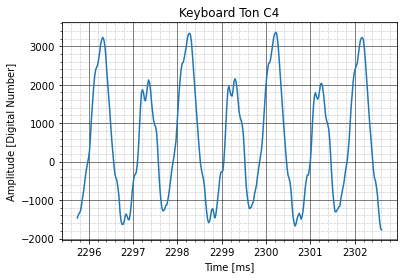
\includegraphics[width=0.5\textwidth]{media/plotDecodedRichtig.png}
	\caption{Ausschnitt vom Signal des Keyboards}
	\label{fig:VERSUCH_1_PERIODEN}
\end{figure}

In der nachfolgenden Abbildung \ref{fig:VERSUCH_1_DR} ist das gesamte aufgenommene Signal zu sehen. Da wir den Ton schon vor Beginn der Aufnahme abgespielt haben, ist kein Einschwingvorgang oder ähnliches zu erkennen.

\begin{figure}[H]
	\centering\small
	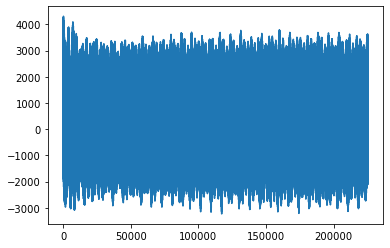
\includegraphics[width=0.5\textwidth]{media/decodedRichtig.png}
	\caption{Das aufgenommene Signal}
	\label{fig:VERSUCH_1_DR}
\end{figure}
\newpage
\section{Auswertung}
\label{chap:VERSUCH_1_AUSWERTUNG}
Aus der Abbildung \ref{fig:VERSUCH_1_PERIODEN} kann die Grundperiode in Millisekunden abgelesen werden, welche 2ms beträgt. Dadurch kann die Grundfrequenz von 500Hz abgeleitet werden. Die Signaldauer, Abtastfrequenz, Signallänge und Abtastintervall können durch einfache Berechnungen ermittelt werden. Die Ergebnisse sind in der Tabelle \ref{fig:VERSUCH_1_AUSWERTUNG_TABELLE} zu sehen.

\begin{table}[H]
\center
\begin{tabular}{|l|l|}
\hline
\multicolumn{1}{|c|}{\textbf{Beschreibung}}   & \textbf{Wert} \\ \hline
Grundperiode {[}ms{]}                         & 2          \\ \hline
Grundfrequenz {[}Hz{]}                        & 500        \\ \hline
Signaldauer {[}sec{]}                         & 5.171     \\ \hline
Abtastfrequenz {[}Hz{]}                       & 43558.89   \\ \hline
Signallänge {[}Anzahl der Abtastzeitpunkte{]} & 225280        \\ \hline
Abtastintervall {[}sec{]}                     & 2.295e-05  \\ \hline
\end{tabular}
\caption{Ergebnisse}
\label{fig:VERSUCH_1_AUSWERTUNG_TABELLE}
\end{table}

Das Amplitudenspektrum wird durch den Betrag der numpy Funktion np.fft.fft() berechnet. Wie zuvor erwähnt, ist die x-Achse Beschriftung jedoch in der Einheit Anzahl Schwingungen innerhalb der gesamten Signaldauer und nicht in Hertz eingegeben. Deshalb muss die oben genannte Formel angewandt werden. Außerdem wird das Amplitudenspektrum nur bis zur Hälfte angezeigt. Dieses wird in Abbildung \ref{fig:VERSUCH_1_ASB} dargestellt.

\begin{figure}[H]
	\centering\small
	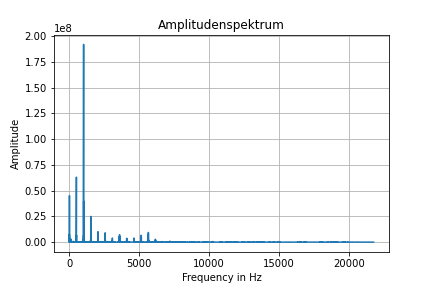
\includegraphics[width=0.5\textwidth]{media/AmplitudenspektrumBreit.png}
	\caption{Gesamtes Amplitudenspektrum bis zur Hälfte}
	\label{fig:VERSUCH_1_ASB}
\end{figure}

\newpage
In Abbildung \ref{fig:VERSUCH_1_ASS} ist ein Ausschnitt des Amplitudenspektrums zu sehen.

\begin{figure}[H]
	\centering\small
	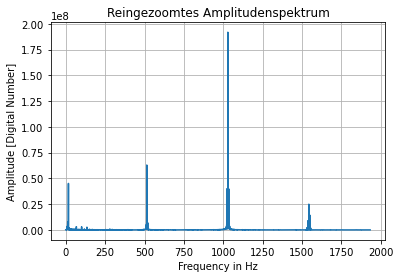
\includegraphics[width=0.5\textwidth]{media/AmplitudenspektrumSchmal.png}
	\caption{Ausschnitt des Amplitudenspektrums}
	\label{fig:VERSUCH_1_ASS}
\end{figure}

Der größte Amplitudenausschlag innerhalb des Spektrums liegt bei der Frequenz 1029Hz. Außerdem ist die Wellenzahl k zu berechnen, die wir mit der Formel 

\begin{equation*}
	k = \frac{1}{\lambda}
\end{equation*}
ermittelt haben. Wobei $\lambda$ die Wellenlänge ist, die in unserem Fall 2ms beträgt. Dies kann in der Abbildung \ref{fig:VERSUCH_1_PERIODEN} abgelesen werden. Durch die errechnete Wellenzahl ergibt sich eine Frequenz von 500Hz, die wiederrum der Grundfrequenz entspricht.


Die Frequenz mit dem maximalen Amplitudenwert kann mithilfe einer einfachen for Schleife, die über das Spektrum iteriert, ermittelt werden.

\begin{table}[H]
\center
\begin{tabular}{|l|l|}
\hline
\multicolumn{1}{|c|}{\textbf{Beschreibung}}   & \textbf{Wert} \\ \hline
Maximaler Amplitudenausschlag                         & 191860000.7          \\ \hline
Frequenz mit der größten Amplitude {[}Hz{]}                        & 1029.22        \\ \hline
\end{tabular}
\caption{Ergebnisse}
\label{fig:VERSUCH_1_MAX}
\end{table}

Der Amplitudenwert bei der Grundfrequenz von 500Hz beträgt ungefähr 0.62 $\cdot$ $10^{8}$ Digital Numbers.

\newpage
\section{Interpretation}
\label{chap:VERSUCH_1_INTERPRETATION}
Wie zu erwarten, ist in Abbildung \ref{fig:VERSUCH_1_PERIODEN} sehr gut ersichtlich, dass der Ton gleichmäßig und mit konstanter Tonhöhe gespielt wurde. 

Aus der Tabelle \ref{fig:VERSUCH_1_AUSWERTUNG_TABELLE} lässt sich schließen, dass die Signaldauer das Ergebnis der Multiplikation von der Signallänge mit dem Abstastintervall ist. Des Weiteren ist das Abtastintervall komplementär zur Abtrastfrequenz, da die Frequenz zunimmt, wenn das Intervall abnimmt. Analog gilt das auch für die Grundperiode und Grundfrequenz.

In Abbildung \ref{fig:VERSUCH_1_ASS} sind die harmonischen vielfachen der Grundfrequenz sehr deutlich zu sehen.
Des Weiteren ist sehr schön zu sehen, dass nicht so viele Obertöne vorhanden sind, was darauf zurückzuführen ist, dass der Ton durch ein digitales Keyboard erzeugt wurde und nicht durch ein klassisches Klavier.

%
% CHAPTER Anhang
%
\renewcommand\thesection{A.\arabic{section}}
\renewcommand\thesubsection{\thesection.\arabic{subsection}}

\chapter*{Anhang}
\label{chap:APPENDIX}
\addcontentsline{toc}{chapter}{Anhang}
%\setcounter{chapter}{0}
\addtocounter{chapter}{1}
\setcounter{section}{0}

\section{Quellcode}
\label{chap:APPENDIX_SOURCECODE}

\subsection{Quellcode Versuch 1}
\label{chap:APPENDIX_SOURCECODE_V1a}
\lstinputlisting[style=PYTHON, frame=single, caption=Skript Versuch 1a, captionpos=b, label=lst:APPENDIX_SOURCECODE_PLOT]{code/Aufgabe1.py}
\label{chap:APPENDIX_SOURCECODE_V1b}
\lstinputlisting[style=PYTHON, frame=single, caption=Skript Versuch 1b, captionpos=b, label=lst:APPENDIX_SOURCECODE_PLOT2]{code/Aufgabe1.2.py}
\label{chap:APPENDIX_SOURCECODE_V1c}
\lstinputlisting[style=PYTHON, frame=single, caption=Skript Versuch 1c, captionpos=b, label=lst:APPENDIX_SOURCECODE_PLOT3]{code/Aufgabe1.3.py}

%
% Literaturverzeichnis
%

\end{document}
%------------------------------------
% ╔═╗╔╗╔╔╦╗  ╔╦╗╔═╗╔═╗╦ ╦╔╦╗╔═╗╔╗╔╔╦╗
% ║╣ ║║║ ║║   ║║║ ║║  ║ ║║║║║╣ ║║║ ║
% ╚═╝╝╚╝═╩╝  ═╩╝╚═╝╚═╝╚═╝╩ ╩╚═╝╝╚╝ ╩
%------------------------------------